\documentclass[dvipsnames,tikz]{standalone}
\usepackage{amsmath}
\usepackage{arevmath}
\usepackage{xcolor}
\usepackage{tikz}
\usetikzlibrary{calc}
\usetikzlibrary{decorations.pathreplacing,calligraphy,3d}
\usepackage{cmbright}      % sansfont

\tikzset{main/.style={draw=black, circle, color=black}}

\begin{document}
	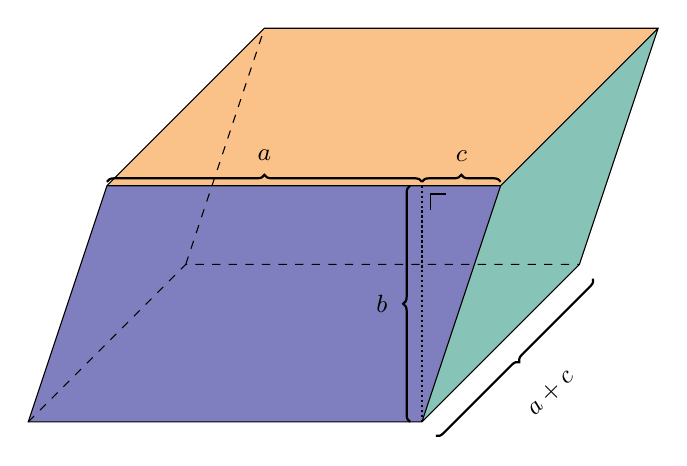
\begin{tikzpicture}[font=\small]
		\fill[BurntOrange, semitransparent] (1,3) --++(5,0) --++(2,2) --++(-5,0) -- cycle;
		\fill[NavyBlue, semitransparent] (1,3) --++(5,0) --++(-1,-3) --++(-5,0) -- cycle;
		\fill[PineGreen, semitransparent] (5,0) --++(2,2) --++(1,3) --++(-2,-2) -- cycle;
		\draw [main] (0,0) -- (5,0) -- (7,2) -- (8,5) -- (3,5) -- (1,3) -- cycle (1,3) -- (6,3) -- (8,5) ++(-2,-2) --++(-1,-3);

		\draw [main, dashed] (0,0) --++ (2,2) --++(5,0) ++(-5,0) --++(1,3);

		\draw[main,densely dotted, thick] (5,0) --++(0,3);
		\begin{scope}[shift={(5,3)}, rotate=-90]
			\draw[main,xshift=3pt, yshift=3pt] (0,0.2) --(0,0) -- (0.2,0);
		\end{scope}
		

		\draw [main, 
			thick,
			decoration={
				brace,
				mirror,
				raise=0.25cm
			},
			decorate
		] (5,0) -- ++(2,2) node [pos=0.5, below, xshift=0.25cm, yshift=-0.25cm, rotate=45] {$a+c$}; 
		\draw [ main,
			thick,
			decoration={
				brace,
				raise=0.05cm
			},
			decorate
		] (1,3) -- ++(4,0) node [pos=0.5, above, yshift=0.1cm] {$a$}; 
		\draw [ main,
			thick,
			decoration={
				brace,
				raise=0.05cm
			},
			decorate
		] (5,3) -- ++(1,0) node [pos=0.5, above, yshift=0.1cm] {$c$}; 

		\draw [ main,
			thick,
			decoration={
				brace,
				raise=0.15cm
			},
			decorate
		] (5,0) -- ++(0,3) node [pos=0.5, left, xshift=-0.2cm] {$b$};
	\end{tikzpicture}
\end{document}